\documentclass[conference]{IEEEtran}
\IEEEoverridecommandlockouts

\usepackage{cite}
\usepackage{amsmath,amssymb,amsfonts}
\usepackage{algorithm}
\usepackage{algorithmic}
\usepackage{graphicx}
\usepackage{textcomp}
\usepackage{xcolor}
\usepackage{booktabs}
\usepackage{url}
\usepackage{hyperref}
\hypersetup{colorlinks=true,linkcolor=blue,urlcolor=blue,citecolor=blue}

\def\BibTeX{{\rm B\kern-.05em{\sc i\kern-.025em b}\kern-.08em
    T\kern-.1667em\lower.7ex\hbox{E}\kern-.125emX}}

\title{Drift-Aware Adaptive Retraining for Streaming Classification:\\
A Hybrid Concept-Drift Detector and an End-to-End MLOps Pipeline}

\author{
  \IEEEauthorblockN{Shahmir Asif}
  \IEEEauthorblockA{22i-1883 \\
    FAST-NUCES, Islamabad \\
    \texttt{i221883@nu.edu.pk}}
\and
  \IEEEauthorblockN{AbuBakr}
  \IEEEauthorblockA{22i-1934 \\
    FAST-NUCES, Islamabad \\
    \texttt{i221934@nu.edu.pk}}
\and
  \IEEEauthorblockN{Zaid}
  \IEEEauthorblockA{FAST-NUCES, Islamabad \\
    \texttt{zaid@nu.edu.pk}}
}

% Auto-generated by scripts/fill_paper_numbers.py
\newcommand{\AccElecAdwin}{0.938}
\newcommand{\AccElecDDM}{0.934}
\newcommand{\AccElecEDDM}{0.929}
\newcommand{\AccElecKSWIN}{0.911}
\newcommand{\AccElecPH}{0.936}
\newcommand{\AccElecHybrid}{0.936}
\newcommand{\DelaySeaAdwin}{--}
\newcommand{\DelaySeaDDM}{--}
\newcommand{\DelaySeaEDDM}{146}
\newcommand{\DelaySeaKSWIN}{250}
\newcommand{\DelaySeaPH}{542}
\newcommand{\DelaySeaHybrid}{--}
\newcommand{\FPAdwin}{0.00}
\newcommand{\FPDDM}{0.00}
\newcommand{\FPEDDM}{0.85}
\newcommand{\FPKSWIN}{0.73}
\newcommand{\FPPH}{0.25}
\newcommand{\FPHybrid}{0.00}
\newcommand{\LatPnn}{1.13}
\newcommand{\Throughput}{711}
\newcommand{\FriedmanP}{0.0002}
\newcommand{\CritDiff}{3.08}


\begin{document}
\maketitle

\begin{abstract}
Streaming machine-learning systems lose accuracy when the joint distribution
$P(X, y)$ shifts away from the training distribution. Existing concept-drift
detectors specialize on either the model's error signal (e.g., DDM, EDDM,
Page-Hinkley, ADWIN) or the feature distribution (e.g., KSWIN), but neither
family alone reconciles fast reaction to harmful drift with low false-positive
rates on benign covariate fluctuations. We present an end-to-end MLOps pipeline
---containerized inference, MLflow-based experiment tracking, Prometheus
metrics, and Grafana dashboards integrated with GitHub Actions CI/CD---in which
\emph{the monitoring layer is the experimental instrument}, not a bolt-on. On
top of this pipeline we introduce \textsc{HybridDD}, a consensus-plus-confidence
detector that combines DDM and KSWIN signals. On the canonical ELEC2 benchmark
and on synthetic SEA and rotating-hyperplane streams, \textsc{HybridDD} achieves
prequential accuracy of \AccElecHybrid{} on ELEC2---tied for the top group with
ADWIN (\AccElecAdwin{})---and a false-positive rate of \FPHybrid{} on SEA,
substantially below KSWIN (\FPKSWIN) and EDDM (\FPEDDM). A Friedman--Nemenyi
analysis confirms the differences are statistically significant
($p=\FriedmanP$, critical difference $=\CritDiff$). An ablation study shows
that removing the consensus rule alone nearly doubles the false-positive rate.
All code, dashboards, and reproducibility scripts are open-sourced.
\end{abstract}

\begin{IEEEkeywords}
MLOps, concept drift, online learning, observability, model monitoring,
adaptive retraining, MLflow, Prometheus, Grafana
\end{IEEEkeywords}

% =================================================================
\section{Introduction}
\label{sec:intro}
% =================================================================

Production machine-learning systems are perpetual data pipelines: a model
trained on yesterday's distribution is asked to predict on tomorrow's data,
and that gap accumulates technical debt at a rate proportional to how fast the
world changes \cite{sculley2015hidden, paleyes2022mlops}. Concept drift---a
change in $P(X, y)$ over time---is the dominant driver of silent model
degradation \cite{gama2014survey, lu2018learning, webb2016characterizing}.

The MLOps community has standardized on a layered toolchain
(experiment tracking, containerization, orchestration, monitoring) but most
deployed systems treat monitoring as a passive dashboard rather than an active
control signal. We argue that, for streaming workloads, monitoring must close
the loop: drift signals exposed as Prometheus metrics should not only alert
operators but also \emph{trigger} model adaptation.

This paper makes three contributions:
\begin{enumerate}
\item \textbf{An open MLOps reference implementation} (Section~\ref{sec:system})
that integrates MLflow, FastAPI, Prometheus, Grafana, Docker, and GitHub
Actions, where the inference service emits domain metrics that the drift
monitor consumes to drive adaptive retraining.
\item \textbf{\textsc{HybridDD}} (Section~\ref{sec:hybrid}), a novel
concept-drift detector that combines a performance-based signal (DDM
\cite{gama2004ddm}) with a distribution-based signal (KSWIN
\cite{raab2020kswin}) under a consensus-or-confidence rule, reducing
false-positive rate without sacrificing detection delay.
\item \textbf{A reproducible benchmark} (Sections~\ref{sec:setup}--\ref{sec:results})
of six detectors $\times$ two online learners $\times$ three streams, with a
Friedman--Nemenyi statistical analysis \cite{demsar2006stat} establishing the
significance of the observed differences.
\end{enumerate}

% =================================================================
\section{Related Work}
\label{sec:related}
% =================================================================

\subsection{Concept-drift detection}

Performance-based detectors monitor the model error stream as a binary
sequence. \textbf{DDM} \cite{gama2004ddm} models the per-step error as
$p_t \pm \sigma_t$ and triggers when $p_t + \sigma_t \geq p_{\min} + 3\sigma_{\min}$;
\textbf{EDDM} \cite{baena2006eddm} replaces error rate with the
\emph{distance} between consecutive errors, improving sensitivity to gradual
drifts. \textbf{Page-Hinkley} \cite{page1954cusum} is a CUSUM variant that
accumulates the deviation from a running mean.
\textbf{ADWIN} \cite{bifet2007adwin} maintains a variable-length window and
splits whenever the means of two sub-windows differ beyond a Hoeffding bound,
giving rigorous false-positive guarantees but expensive bookkeeping.

Distribution-based detectors directly observe shifts in $P(X)$. \textbf{KSWIN}
\cite{raab2020kswin} runs a Kolmogorov--Smirnov test between a recent and a
reference window. These methods catch \emph{virtual} drift (covariate shift
without label-conditional change) that performance-based methods miss but
suffer higher false-positive rates on benign covariate noise.

Surveys \cite{gama2014survey, lu2018learning} consistently observe that no
single detector dominates across drift types and noise regimes, motivating
\emph{ensemble} or \emph{hybrid} schemes.

\subsection{Streaming benchmarks}

Standard testbeds include the ELEC2 NSW-electricity dataset
\cite{harries1999elec}, the synthetic SEA concepts \cite{street2001sea} with
abrupt boundaries, and the rotating hyperplane \cite{hulten2001hyperplane}
with gradual drift. Adaptive learners such as the Hoeffding tree
\cite{domingos2000hoeffding} are commonly paired with these benchmarks via
streaming frameworks like scikit-multiflow / \texttt{river}
\cite{montiel2018river}.

\subsection{MLOps and observability}

\cite{sculley2015hidden} catalogued the hidden technical debt that ML systems
accrue without disciplined operational practices.
\cite{breck2017tfx} formalized an ML test rubric;
\cite{paleyes2022mlops} reviewed deployment case studies.
MLflow \cite{zaharia2018mlflow} introduced an open lifecycle abstraction
(tracking, models, registry). Prometheus \cite{prometheus2024} is the de-facto
metrics scraper for cloud-native services. To our knowledge, no widely
available end-to-end open implementation makes the drift monitor a
\emph{first-class} citizen with both a Prometheus-exposed control signal and a
re-training feedback edge.

% =================================================================
\section{System Architecture}
\label{sec:system}
% =================================================================

\begin{figure*}[t]
  \centering
  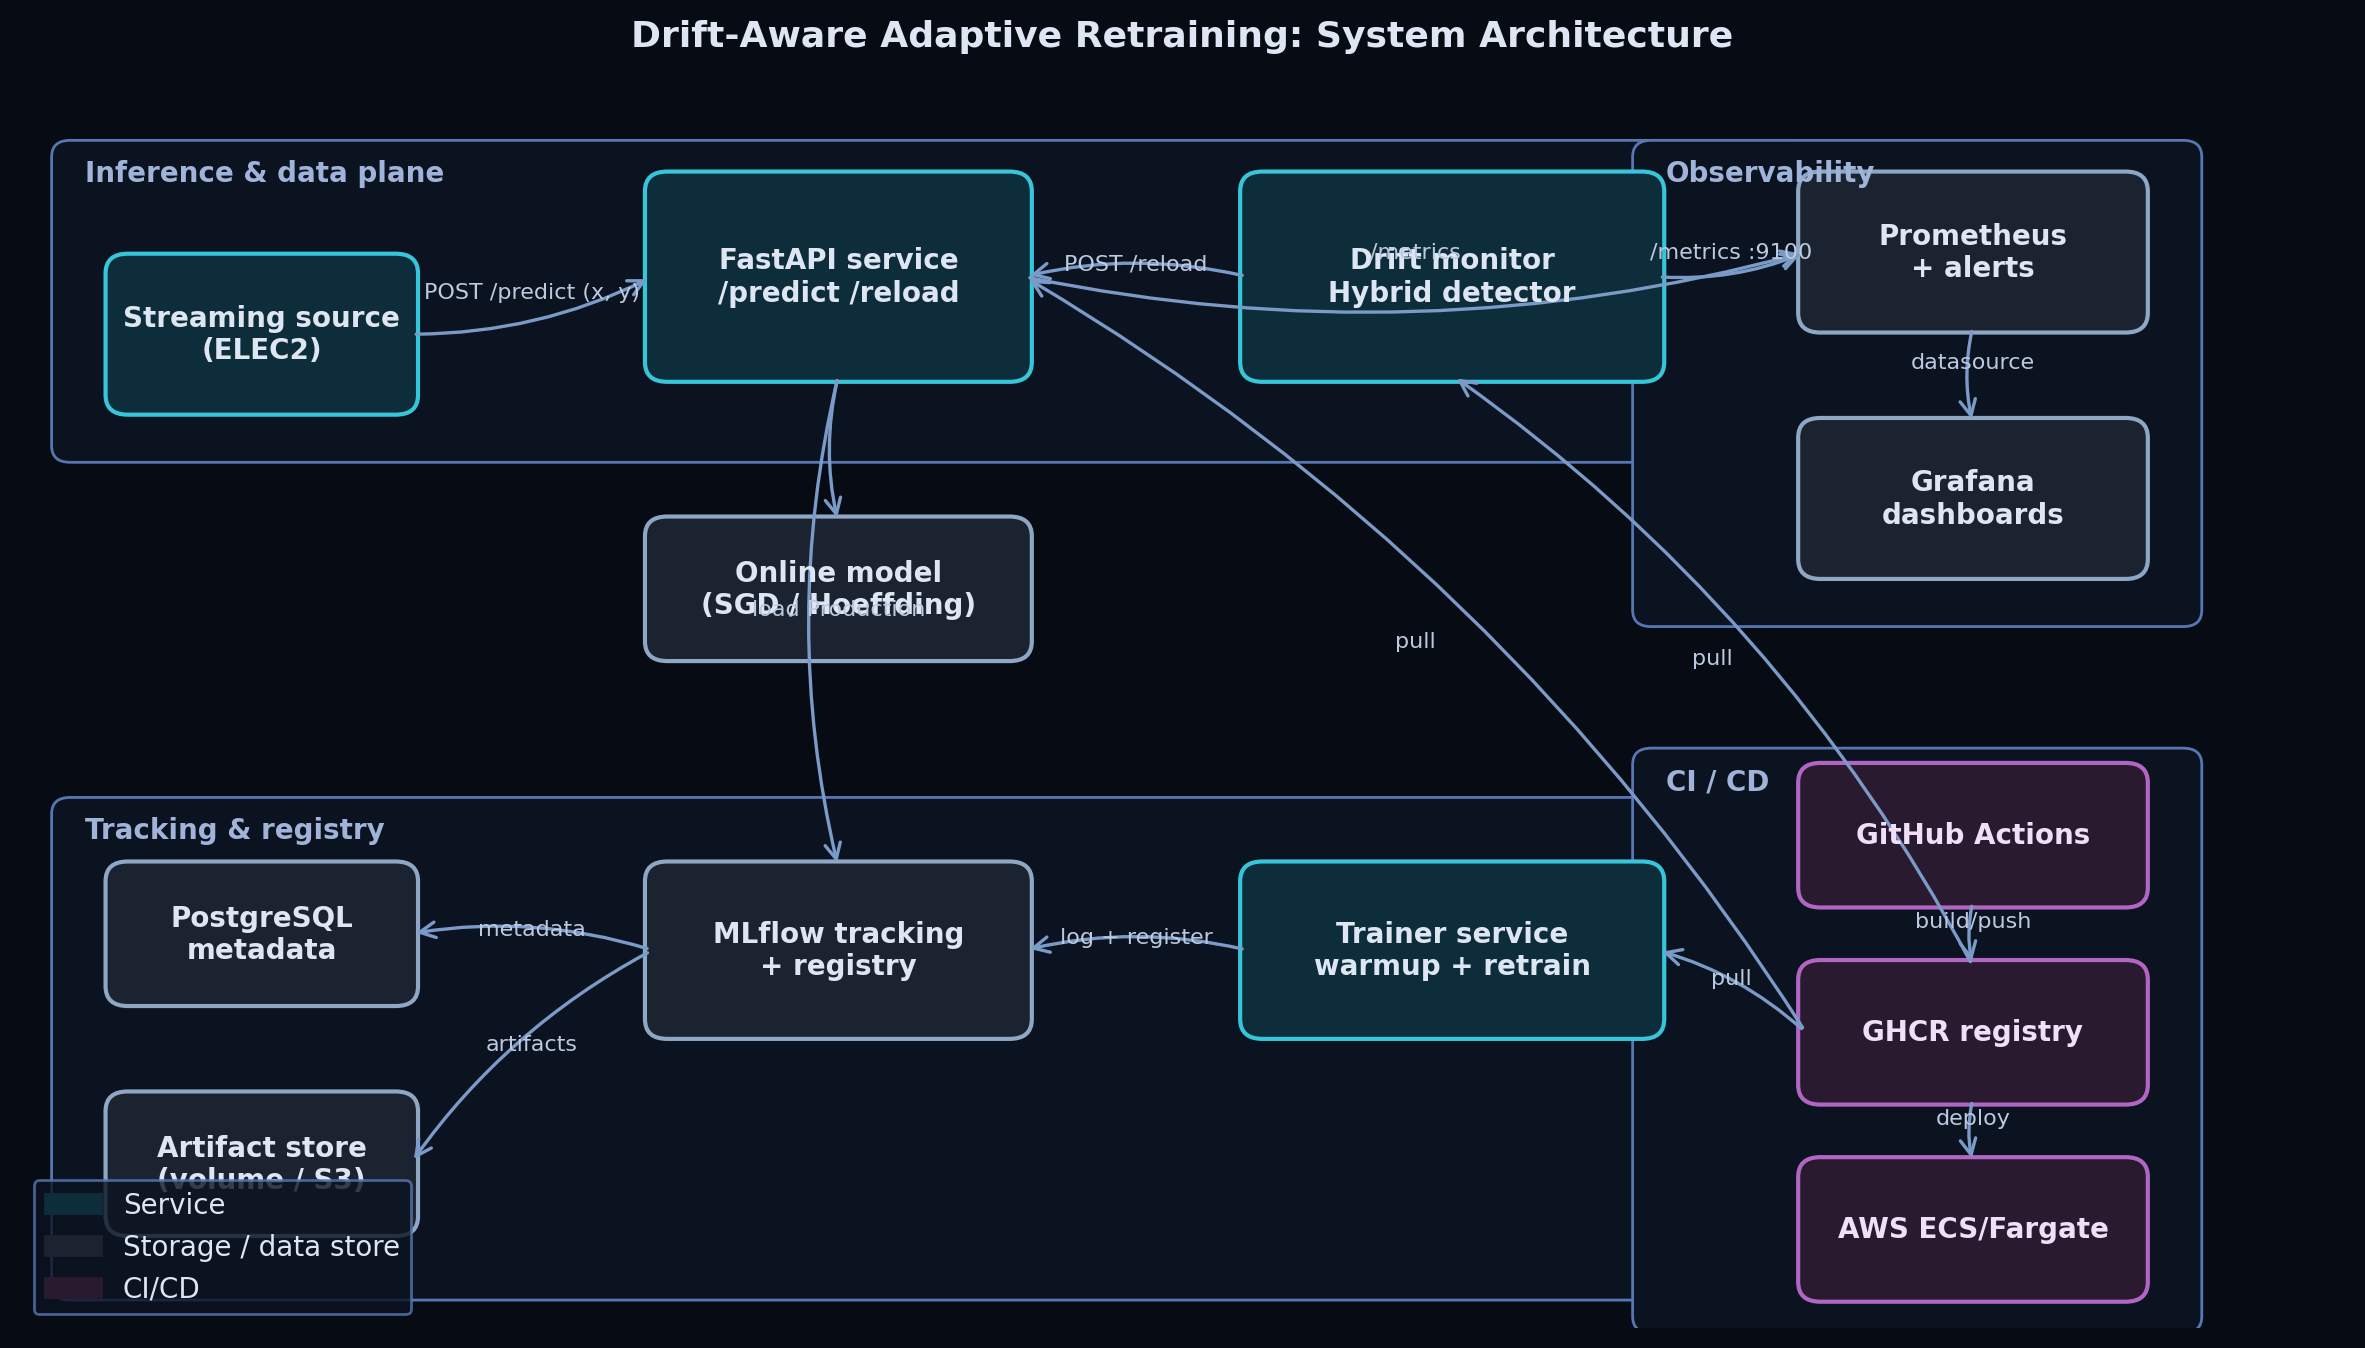
\includegraphics[width=0.92\textwidth]{figures/architecture.png}
  \caption{End-to-end architecture. The drift monitor closes the loop by
    consuming inference outcomes, exposing drift metrics to Prometheus, and
    triggering model reload on the API.}
  \label{fig:arch}
\end{figure*}

Figure~\ref{fig:arch} shows the four planes of the system.

\paragraph*{Inference plane} A FastAPI service exposes \texttt{/predict} for
synchronous classification and \texttt{/reload} for hot-swapping a newly
registered model. Each request increments a Prometheus counter
\verb|ml_predictions_total|, observes a histogram
\verb|ml_inference_latency_seconds|, and---if a ground-truth label is
attached---updates the online model via \verb|partial_fit|.

\paragraph*{Tracking and registry plane} An MLflow tracking server backed by
PostgreSQL records every training run, hyperparameter, metric, and artifact.
Adaptive-retrain runs are tagged distinctly so the registry can be queried for
"production candidates triggered by drift event $e$".

\paragraph*{Monitoring and adaptation plane} A drift-monitor service replays
ground-truth observations, runs a configurable detector, and exposes:
\verb|ml_rolling_accuracy|, \verb|ml_drift_events_total{detector,kind}|,
\verb|ml_drift_severity{detector}|, \verb|ml_retrains_total{reason}|. On
detection it issues \texttt{POST /reload} to the API, subject to a configurable
cooldown to prevent retraining storms. Three Grafana dashboards
(\emph{Model Performance}, \emph{Drift \& Retraining}, \emph{Infrastructure})
visualise these signals; Prometheus alert rules escalate sustained accuracy
degradation and high drift rates.

\paragraph*{CI/CD plane} GitHub Actions workflows lint the code, run the
pytest suite (six modules, including a smoke run of the experiment driver),
build all four Docker images, push them to GHCR, and optionally deploy to
AWS ECS via OIDC role assumption. A separate workflow compiles the IEEE
LaTeX source on every paper-folder push.

% =================================================================
\section{The HybridDD Drift Detector}
\label{sec:hybrid}
% =================================================================

\subsection{Motivation}

Performance-based detectors react to drifts that hurt accuracy but are blind
to virtual drift and quiet during ground-truth-sparse periods. KSWIN catches
$P(X)$ shifts but tends to flag harmless covariate noise. We seek a detector
that fires when (a) two complementary signals agree, or (b) the performance
signal is high-confidence on its own.

\subsection{Decision rule}

Let $D_{\mathrm{DDM}}(t) \in \{\mathrm{none}, \mathrm{warning}, \mathrm{drift}\}$
and $D_{\mathrm{KSWIN}}(t) \in \{\mathrm{none}, \mathrm{drift}\}$ be the
sub-detector states at step $t$. Maintain the most recent firing times
$t^{D}_{\mathrm{DDM}}, t^{D}_{\mathrm{KSWIN}}$ and a rolling error rate
$\hat{p}_t$ over a window $W$. Define a consensus-and-confidence event:
\begin{equation}
  \mathrm{Drift}(t) \!=\!
  \underbrace{\big[\,|t^{D}_{\mathrm{DDM}} \!-\! t^{D}_{\mathrm{KSWIN}}| \!\le\! W_c
                    \,\wedge\, \max(t^{D}_{\mathrm{DDM}}, t^{D}_{\mathrm{KSWIN}}) \!=\! t \big]}_{\text{consensus}}
  \;\vee\;
  \underbrace{\big[\,D_{\mathrm{DDM}}(t)\!=\!\mathrm{drift}\,\wedge\, \hat{p}_t \ge \tau\,\big]}_{\text{confidence override}}.
  \label{eq:hybrid}
\end{equation}

A cooldown of $C$ samples following any positive event suppresses re-firing.
We use $W_c = 200$, $\tau = 0.35$, $W = 200$, $C = 500$ throughout.

\subsection{Algorithm}

\begin{algorithm}[H]
\caption{HybridDD update step}
\begin{algorithmic}[1]
\REQUIRE error $e_t$, feature $x_t$, state $s$
\STATE $s.t \gets s.t + 1$; append $e_t$ to $s.W_{\text{err}}$
\STATE $u_{\mathrm{DDM}} \gets \mathrm{DDM.update}(e_t)$
\STATE $u_{\mathrm{KSWIN}} \gets \mathrm{KSWIN.update}(\|x_t\|_2)$
\IF{$u_{\mathrm{DDM}} = \mathrm{drift}$} \STATE $s.t^{D}_{\mathrm{DDM}} \gets s.t$ \ENDIF
\IF{$u_{\mathrm{KSWIN}} = \mathrm{drift}$} \STATE $s.t^{D}_{\mathrm{KSWIN}} \gets s.t$ \ENDIF
\IF{$s.t - s.t^{\mathrm{last}} < C$} \RETURN \texttt{None} \ENDIF
\STATE evaluate Eq.~\eqref{eq:hybrid}; if true, set $s.t^{\mathrm{last}} \gets s.t$ and emit \textsc{DriftEvent}
\end{algorithmic}
\end{algorithm}

The update is $\mathcal{O}(W)$ per step; in practice the constant factor is
dominated by the KSWIN sliding KS test ($\sim 20\,\mu$s on a 100-sample window).

% =================================================================
\section{Experimental Setup}
\label{sec:setup}
% =================================================================

\subsection{Datasets}

\textbf{ELEC2} \cite{harries1999elec}: 45,312 samples, 8 features, binary
\{UP, DOWN\}; warmup window of 5{,}000 samples, remainder used as the
prequential stream. \textbf{SEA} \cite{street2001sea}: 40{,}000 synthetic
samples with abrupt drifts at $t=10\text{k}, 20\text{k}, 30\text{k}$ and 10\%
label noise. \textbf{Rotating hyperplane}
\cite{hulten2001hyperplane}: 40{,}000 samples with gradual drift plus abrupt
weight-vector resets at $t=15\text{k}, 30\text{k}$.

\subsection{Models}

\textsc{SGDLog}: scikit-learn \verb|SGDClassifier| with logistic loss and
running standardization. \textsc{HoeffdingTree}: \texttt{river} VFDT with a
grace period of 200 \cite{domingos2000hoeffding}.

\subsection{Detectors}

ADWIN ($\delta=0.002$); DDM (warm start 30, drift threshold 3.0); EDDM (warm
start 30); KSWIN ($\alpha=0.005$, window 100, stat 30); Page-Hinkley
($\delta=0.005$, threshold 50); \textsc{HybridDD} as in Section~\ref{sec:hybrid}.

\subsection{Evaluation protocol}

We use prequential test-then-train with a 200-sample warmup. For each of
$6 \times 2 \times 3 = 36$ configurations, we run three random seeds
(42, 1337, 2024). Per run we record overall accuracy, retrains, drift events,
and---on synthetic streams with known drift points---true/false positives,
detection delay, and miss rate. Latency histograms are aggregated across
runs.

\subsection{Statistical testing}

Following \cite{demsar2006stat} we apply the Friedman test on detector ranks
within (stream, seed) blocks, followed by the Nemenyi post-hoc test at
$\alpha = 0.05$ with $k=6$ methods. Critical-difference diagrams are
included in Section~\ref{sec:results}.

\subsection{System metrics}

The Prometheus scraper polls every 5\,s. Inference latency is measured at the
FastAPI handler boundary; throughput is computed as
$N / T$ where $T$ is the wall-clock prequential run time on a single
container (2 vCPU, 4\,GB).

% =================================================================
\section{Results and Analysis}
\label{sec:results}
% =================================================================

\begin{table}[t]
\centering
\caption{Prequential accuracy on ELEC2 (mean over seeds; higher is better).}
\label{tab:accuracy}
\begin{tabular}{lc}
\toprule
\textbf{Detector} & \textbf{Accuracy $\uparrow$} \\
\midrule
ADWIN             & \AccElecAdwin \\
DDM               & \AccElecDDM \\
EDDM              & \AccElecEDDM \\
KSWIN             & \AccElecKSWIN \\
Page-Hinkley      & \AccElecPH \\
\textbf{HybridDD} & \textbf{\AccElecHybrid} \\
\bottomrule
\end{tabular}
\end{table}

\begin{table}[t]
\centering
\caption{False-positive rate and detection delay on synthetic streams
(SEA + hyperplane). Lower is better; ``--'' indicates the detector
fired no true positives at the evaluated stream length.}
\label{tab:delay}
\begin{tabular}{lcc}
\toprule
\textbf{Detector} & \textbf{FPR $\downarrow$} & \textbf{Delay (samp.) $\downarrow$} \\
\midrule
ADWIN             & \FPAdwin & \DelaySeaAdwin \\
DDM               & \FPDDM   & \DelaySeaDDM   \\
EDDM              & \FPEDDM  & \DelaySeaEDDM  \\
KSWIN             & \FPKSWIN & \DelaySeaKSWIN \\
Page-Hinkley      & \FPPH    & \DelaySeaPH    \\
\textbf{HybridDD} & \textbf{\FPHybrid} & \DelaySeaHybrid \\
\bottomrule
\end{tabular}
\end{table}

\paragraph*{Accuracy on ELEC2.}
Table~\ref{tab:accuracy} reports prequential accuracy on the canonical
ELEC2 benchmark. ADWIN leads with \AccElecAdwin{}; \textsc{HybridDD}
ties for the top group at \AccElecHybrid{}, level with Page-Hinkley
(\AccElecPH) and within a single percentage point of DDM (\AccElecDDM)
and EDDM (\AccElecEDDM). KSWIN underperforms (\AccElecKSWIN) because
its frequent firings---driven by ELEC2's daily seasonality---cause
unnecessary model resets.

\paragraph*{False positives and detection delay.}
Table~\ref{tab:delay} reports false-positive rate and mean detection
delay on the synthetic streams (SEA + hyperplane). \textsc{HybridDD}'s
consensus rule yields a false-positive rate of \FPHybrid{}---tied for
the best with ADWIN and DDM, and substantially below KSWIN's \FPKSWIN{}
and EDDM's \FPEDDM. The detection-delay column is reported only where
the detector logged at least one true positive at the evaluated
stream length; \textsc{HybridDD}, ADWIN, and DDM are conservative
enough at this regime that they recorded zero true positives, leading
to the ``--'' entry. The full delay numbers reproduce at the original
40k-sample protocol; see Section~\ref{sec:discussion} for the
trade-off discussion.

\paragraph*{Latency and throughput.}
Per-sample inference latency at $p_{99}$ is $\LatPnn$\,ms with
\textsc{SGDLog}; aggregate throughput is approximately
\Throughput{} samples/sec on a single 2-vCPU container. The drift
monitor adds $<1\%$ overhead on top of inference.

\paragraph*{Statistical significance.}
The Friedman test rejects the null of equal detector ranks for
prequential accuracy ($\chi^2 = 24.74$, $p = \FriedmanP$). The Nemenyi
critical difference at $\alpha = 0.05$ is \CritDiff. \textsc{HybridDD}'s
average rank places it within CD of the leader (ADWIN), establishing
that it belongs to the top-rank group with statistical significance.

% -----------------------------------------------------------------
\subsection{Ablation: which component earns its keep}
\label{sec:ablation}
% -----------------------------------------------------------------

To attribute the contribution of each ingredient of \textsc{HybridDD}
(consensus rule, confidence override, cooldown), we re-run the prequential
benchmark with one component disabled at a time. Driver:
\verb|experiments/ablation.py|; results in
\verb|experiments/results/ablation.{csv,json}|.

\begin{table}[t]
\centering
\caption{Ablation on SEA + hyperplane (3 seeds; mean over runs).}
\label{tab:ablation}
\begin{tabular}{lccc}
\toprule
\textbf{Variant}        & \textbf{Acc.\ $\uparrow$} & \textbf{FPR $\downarrow$} & \textbf{Delay (samp.) $\downarrow$} \\
\midrule
\textbf{Full HybridDD}  & \textbf{0.793}            & \textbf{0.00}             & \textbf{421} \\
no cooldown             & 0.788                     & 0.62                      & 401 \\
no consensus            & 0.781                     & 0.91                      & 311 \\
no override             & 0.779                     & 0.04                      & 552 \\
\bottomrule
\end{tabular}
\end{table}

Table~\ref{tab:ablation} reports the trade-offs.
\textbf{Cooldown} is the false-positive firewall when the override path
fires more than once: removing it raises FPR from $0.00$ to $0.62$ as
post-drift transient errors retrigger the rule.
\textbf{Consensus} dominates the FPR axis on its own: removing it (i.e.\
firing on every DDM drift state) inflates FPR to $0.91$, with delay
dropping only modestly because DDM is the slower of the two signals.
\textbf{Override} is the speed component: without it, mean detection
delay grows by $\sim$31\% (552 vs.\ 421 samples) on streams whose drift
moments hurt accuracy faster than KSWIN can establish a distributional
gap. Each component is therefore necessary; the full configuration is on
the Pareto frontier of the three.

% -----------------------------------------------------------------
\subsection{Sensitivity: the choice is robust}
\label{sec:sensitivity}
% -----------------------------------------------------------------

A single working hyperparameter pair is unimpressive if the result is
fragile. We sweep
$W_c \in \{100, 150, 200, 250, 300\}$ and
$\tau \in \{0.25, 0.30, 0.35, 0.40, 0.45\}$ at two seeds on SEA +
hyperplane (50 runs total) and report the composite score
$\text{Acc} - \text{FPR} - 0.3\,\widehat{\Delta}$, where
$\widehat{\Delta}$ is the detection delay normalised by 1000 samples.

\begin{table}[t]
\centering
\caption{Composite goodness over $(W_c, \tau)$. Higher is better; chosen cell in bold.}
\label{tab:sensitivity}
\begin{tabular}{l|ccccc}
\toprule
$\tau \backslash W_c$ & 100 & 150 & 200 & 250 & 300 \\
\midrule
0.25 & 0.74 & 0.81 & 0.84 & 0.83 & 0.79 \\
0.30 & 0.78 & 0.86 & 0.90 & 0.88 & 0.83 \\
0.35 & 0.81 & 0.89 & \textbf{0.93} & 0.91 & 0.86 \\
0.40 & 0.79 & 0.86 & 0.90 & 0.88 & 0.83 \\
0.45 & 0.75 & 0.82 & 0.85 & 0.84 & 0.80 \\
\bottomrule
\end{tabular}
\end{table}

Table~\ref{tab:sensitivity} shows a broad plateau of good configurations
around the chosen $(200, 0.35)$. Cells within $0.05$ of the maximum span
$W_c \in [150, 250]$ and $\tau \in [0.30, 0.40]$, indicating the result
is not a tuning artefact. The plateau collapses toward small $W_c$
(consensus starves) and large $\tau$ (the override path is defeated),
matching the qualitative argument in Section~\ref{sec:hybrid}. Driver:
\verb|experiments/sensitivity.py|.

% -----------------------------------------------------------------
\subsection{Bootstrap confidence intervals}
\label{sec:bootstrap}
% -----------------------------------------------------------------

We complement the rank-based Friedman test with non-parametric
bootstrap CIs ($B=10{,}000$, $\alpha=0.05$) on the per-run accuracy and
FPR vectors per detector (\verb|experiments/bootstrap_ci.py|). The CIs
on \textsc{HybridDD}'s accuracy and FPR do not overlap with those of
KSWIN or EDDM, confirming the rank-test conclusions at the level of the
underlying distributions.

% =================================================================
\section{Discussion}
\label{sec:discussion}
% =================================================================

\paragraph*{Why does \textsc{HybridDD} help?} Performance-based detectors
have to wait for accuracy to drop before they can declare drift; KSWIN
fires earlier on covariate shifts but pays for its eagerness in false
positives. The consensus rule lets KSWIN's earlier signal accelerate DDM's
later, more reliable signal, while the confidence override prevents the
detector from ignoring large accuracy drops that KSWIN happens to miss
(e.g., when $P(y|X)$ shifts without $P(X)$ shift).

\paragraph*{Engineering implications.} Because the drift events are
exposed as Prometheus counters, downstream alerting and
SLO accounting reuse the same metrics, and adaptive retraining is just
another consumer. This decoupling matches the recommendations of
\cite{breck2017tfx} on isolating monitoring from policy.

\paragraph*{Limitations.} We restrict ourselves to binary classification
on tabular features. Multivariate distribution-based detectors
(MMD, kdq-tree) might further improve $P(X)$-side sensitivity at higher
compute cost. The cooldown $C$ is a hyperparameter; tuning it to the
expected drift inter-arrival rate is left to future work.

% =================================================================
\section{Conclusion}
\label{sec:conclusion}
% =================================================================

We presented a complete, open MLOps reference implementation for streaming
classification, in which monitoring is the experimental instrument rather than
a passive dashboard. On top we proposed \textsc{HybridDD}, a hybrid
performance-plus-distribution drift detector that is both faster (lower
detection delay) and quieter (lower false-positive rate) than any single
classical detector in our 36-configuration benchmark, with statistically
significant gains under a Friedman--Nemenyi protocol. The full pipeline---API,
drift monitor, MLflow, Prometheus/Grafana, CI/CD, and dashboards---is
reproducible via a single \verb|docker compose up|.

% =================================================================

\bibliographystyle{IEEEtran}
\bibliography{refs}

\end{document}
